\documentclass{article}

\usepackage[margin=2.5cm,left=2cm,includefoot]{geometry}
\usepackage{graphicx}
\usepackage{float}
\usepackage[space]{grffile}
\usepackage{hyperref}
\usepackage[export]{adjustbox}
\usepackage{multicol}
\usepackage{caption}
\usepackage{hyperref}
\usepackage{listings}
\usepackage{vhistory}
\usepackage{titlesec}

\setcounter{secnumdepth}{4}

\titleformat{\paragraph}
{\normalfont\normalsize\bfseries}{\theparagraph}{1em}{}
\titlespacing*{\paragraph}
{0pt}{3.25ex plus 1ex minus .2ex}{1.5ex plus .2ex}

% Header and footer
\usepackage{fancyhdr}
\pagestyle{fancy}

\rhead{COS301}
\lhead{User Manual Document}
\fancyfoot[R]{Page \thepage}

\renewcommand{\headrulewidth}{2pt}
\renewcommand{\footrulewidth}{1pt}

\begin{document}

	\begin{titlepage}
		\begin{center}
			
\includegraphics[width=10cm]{images/UP.jpg}  \\
			[0.5cm]
			\huge{
			User Manual Document\\
			}
			
			\line(1,0){300}\\
			[0.2cm]
			\LARGE{Project: MarketLead.io\\
			Client: RetroRabbit} \\
			\line(1,0){300}\\
			\LARGE{Team: Valknut Solutions}\\
			[1.0cm]
			\large{Version: 1.1}\\
			[1.0cm]
			\large
			{
			\begin{itemize}
				\item 13054903 - Charl Jansen van Vuuren 
				\item 10297902 - Bernhard Schuld      
				\item 13044924 - Kevin Heritage
				\item 13176545 - Quinton Weenink\\
			\end{itemize}
			}
			\textsc{\large}\\
		[3.0cm]
		\textsc{\large  Department of Computer Science}\\
		[0.5cm]
		\textsc{\large \today}\\
		\end{center}
	\end{titlepage}
	
	\cleardoublepage
	% Start of the revision history table
	\begin{versionhistory}
  		\vhEntry{1.0}{27.7.2016}{CJvV,KH,QW}{in progress}
  		\vhEntry{1.1}{9.9.2016}{CJvV,KH,QW}{Changed Project name. Updates for new use cases and modules}
	\end{versionhistory}	
	
	\cleardoublepage
	\tableofcontents
	\cleardoublepage
	
	\section{General Information}
		\subsection{System Overview}
			This document contains information related to the use of the MarketLead.io system that is being developed for RetroRabbit as part of the COS301 module at the University Of Pretoria. 
			The purpose of the system is to gather information from various social media platforms. The data that was gathered can then be visualized in graphs for analysts.
			Users that are interested with a product that the system has to offer does not necessarily work with the system directly but rather through the various social media platforms.
			A marketer can register their different social media platforms to interact with the system through the website.
			This user manual is not for the clients/users on the social media platforms rather for the analysts and marketers that physically interact with the system.

		\subsection{System Configuration}
			The main input of data to the system will be from the various social media platforms from clients. Marketers and analysts will use the web interface to use the system.

	\section{Getting Started}
		A user/client needs to be signed up for the various social media platforms that the system uses.
		Marketers should also have accounts at the various social media platforms.
		Analysts will receive a login from an administrator of the system to be able to log into the system and see analytics.\\
		Marketers and analysts can open their web browser (Mozilla Firefox/Chrome recommended) and go to \href{https://insuranceprofiling.herokuapp.com}{MarketLead.io} to get started with their various tasks.
		When the marketer/analyst is done using the system they can simply close the web browser window to end their session with the system.

	\section{Using the system}
		\subsection{Signing up your page}
			This section will cover the steps necessary for signing up your Facebook page in order for Facebook to send the data from the Lead Ads on your page through to the Insurance profiling server for processing.
			\begin{enumerate}
				\item Navigate to the website\\
				Open up the browser of your choice (Mozilla Firefox recommended) and navigate to the \href{https://insuranceprofiling.herokuapp.com}{Insurance Profiling} website.

				\item Sign up\\
				Click on the Sign Up button in the top right corner of the website\\
				\begin{figure}[H]
				  \centering
				      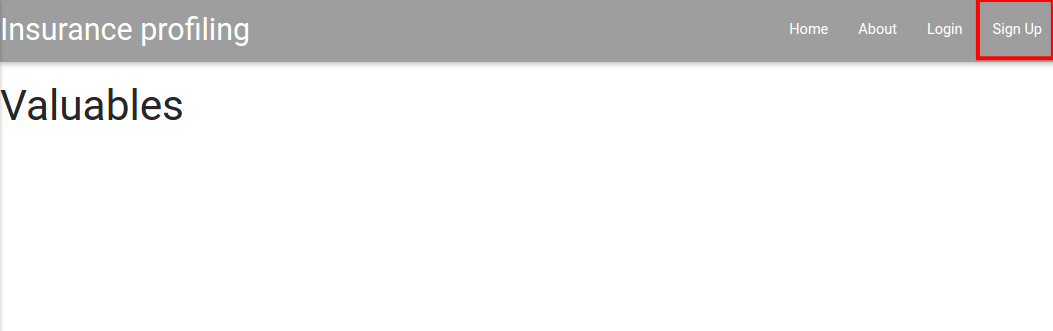
\includegraphics[width=\textwidth]{images/home_signup.png}
				  \caption{Home page indicating where to sign up}
				  \label{fig:homeSignup}
				\end{figure}

				\item Login with Facebook\\
				Once redirected click the button to Login with Facebook\\
				\begin{figure}[H]
				  \centering
				      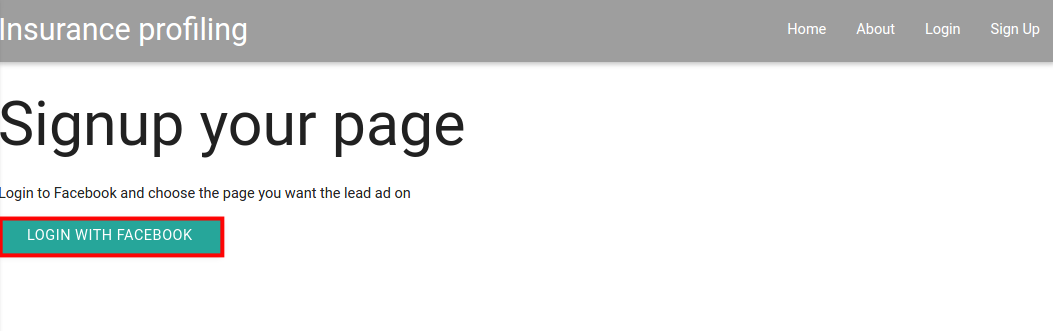
\includegraphics[width=\textwidth]{images/signup_login.png}
				  \caption{Button to click to login with Facebook}
				  \label{fig:signupLogin}
				\end{figure}
				When you have clicked the button a pop-up will appear requesting you to log into Facebook requesting permissions for the system to manage your pages.

			\item Selecting the page to manage\\
				Once the user has logged into their Facebook account with permission to manage their pages, a list of their pages will be displayed.\\
				Select the page that the system needs to manage.\\
				\begin{figure}[H]
				  \centering
				      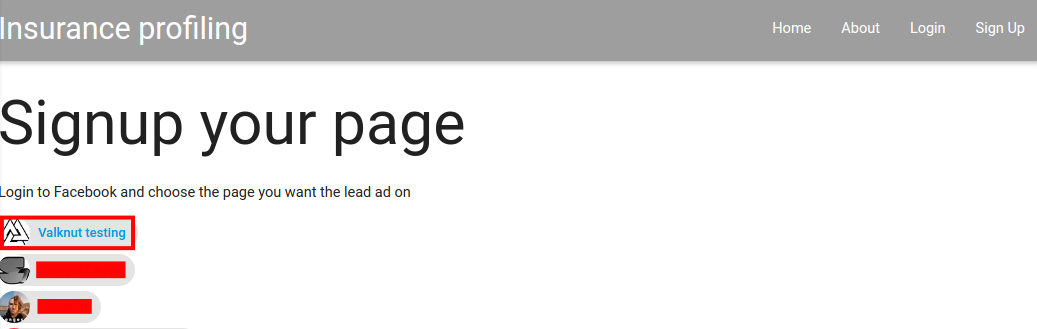
\includegraphics[width=\textwidth]{images/select_page.png}
				  \caption{Selecting the page to manage}
				  \label{fig:selectPage}
				\end{figure}
				When clicking on the page that the system should manage the user can create a lead ad.\\
				To create a lead ad user this Facebook references: \href{https://www.facebook.com/business/a/lead-ads}{Facebook Lead adverts}
			\end{enumerate}
	
	\section{Troubleshooting}

	\section{References to other documentation}
		\begin{itemize}
			\item{Requirements specifications as per 29 July 2016}
			\item{Architecture Design as per 29 July 2016}
			\item{\href{https://www.facebook.com/business/a/lead-ads}{Facebook Lead adverts} as per 29 July 2016}
		\end{itemize}

\end{document}
